% 05_power_spectrum.tex
\section{The CMB angular power spectra}
\label{ch:cls}

We now assemble everything into the observable: the angular power spectrum $C_\ell$. The pipeline is a single sentence: evolve the perturbations for every $k$, build source functions, do the LOS integral against $j_\ell$, integrate against the primordial power spectrum, normalise. This chapter executes that sentence and validates the result against CAMB.

\subsection{The master formula}

The CMB temperature on our sky is a stochastic field. Its statistical properties are summarised by the angular power spectrum
\[
  C_\ell^{XY} = \langle a^X_{\ell m}\, a^{Y*}_{\ell m}\rangle,
\]
with $a^X_{\ell m}$ the spherical-harmonic coefficients of the relevant field ($X \in \{T, E\}$ for us). Going through the projection from $\vec k$-space to the sky, the result is
\begin{equation}
  C_\ell^{XY} = 4\pi \int_0^\infty \frac{\mathrm{d}k}{k}\, \mathcal{P}_\mathcal{R}(k)\, \Delta_\ell^X(k)\, \Delta_\ell^Y(k),
  \label{eq:Cl_master}
\end{equation}
with $\mathcal{P}_\mathcal{R}(k) = A_s (k/k_*)^{n_s - 1}$ the dimensionless primordial curvature power spectrum and $\Delta_\ell^X(k)$ the transfer functions from chapter 4. The factor of $4\pi$ comes from the spherical-harmonic normalisation; the $\mathrm{d}k/k$ measure is natural because primordial perturbations are scale-invariant to a good approximation.

For $E$-mode polarisation the master formula picks up an extra normalisation, $\sqrt{(\ell+2)!/(\ell-2)!}$, from the spin-2 differential operator -- this factor sits inside our \texttt{compute\_spectra} function as \texttt{ctnorm}.

We usually report not $C_\ell$ itself but
\[
  \mathcal{D}_\ell^{XY} = \frac{\ell(\ell + 1)}{2\pi}\, C_\ell^{XY},
\]
which is approximately flat on the Sachs-Wolfe plateau.

\subsection{Anatomy of the spectrum}

Before plotting, it is worth knowing what to expect at each scale.

\paragraph{Sachs-Wolfe plateau ($\ell \lesssim 30$).}
At these scales the modes are still super-horizon at last scattering. The dominant contribution is $\Theta_0 + \Psi_W \approx \tfrac{1}{3}\Psi_W$ (the classic SW formula), which freezes out at horizon crossing. Result: $\mathcal{D}_\ell \approx \mathrm{const}$, with amplitude set by $A_s$.

\paragraph{Acoustic peaks ($30 \lesssim \ell \lesssim 1000$).}
Modes that completed an integer number of oscillation half-cycles by last scattering produce extrema in $\delta_\gamma + 4\Psi_W$. The $n$-th compression peak (odd $n$) is enhanced by baryon mass and the $n$-th rarefaction peak (even $n$) is suppressed: the even/odd ratio measures $\omega_b$. The angular position of the first peak,
\[
  \ell_1 \approx \pi\,\chi_*/r_s \approx 220,
\]
measures the angular scale of the sound horizon and fixes the geometry.

\paragraph{Silk damping tail ($\ell \gtrsim 1000$).}
Photon diffusion smears small-scale anisotropies on a comoving scale $\lambda_D = 1/k_D$, producing an exponential damping envelope $e^{-(\ell/\ell_D)^2}$ with $\ell_D \sim k_D \chi_* \sim 1500$.

\paragraph{Reionisation bump on EE ($\ell \lesssim 10$).}
Reionisation scatters CMB photons off late-time free electrons. Because polarisation is generated only by an anisotropic radiation field, the contribution is amplified relative to TT. This produces a low-$\ell$ EE bump that measures $\tau_\mathrm{reion}$.

\subsection{Choice of grids}

For the LOS integral and the $\int \mathrm{d}\ln k$ integral we need two $k$-grids: a coarse grid for the ODE evolution (the Boltzmann hierarchy is smooth in $k$, $\sim 100$-$200$ modes suffice) and a fine grid for the LOS integral (the transfer function $\Delta_\ell(k)$ oscillates rapidly, so we need $\sim 4000$ modes). For the time integral we need a $\tau$-grid concentrated near recombination (where the visibility function lives) and near reionisation. Both grids are constructed by an equidistribution principle: the node density is proportional to $|f''|^{1/3}$ of an estimator function, which minimises trapezoidal-rule error.

\subsection{The code: \texttt{make\_k\_grid}}

\begin{codebox}[Cell: \texttt{make\_k\_grid}]
\begin{lstlisting}[style=python]
def make_k_grid(N, mode, bg, thermo, params,
                k_min=1e-5, k_max=0.5,
                ell_min=2, ell_max=2500, n_ell_samples=30,
                n_eval=5000):
    """Optimal non-uniform k-grid.
    mode='cl'  : optimised for the C_ell integral
    mode='ode' : optimised for source-function interpolation.
    """
    x = np.linspace(np.log(k_min), np.log(k_max), n_eval)
    k = np.exp(x)
    primordial    = k ** (params['n_s'] + 2)
    acoustic_curv = (1.0 / thermo['r_s']) ** 2

    if mode == "cl":
        damped   = primordial * np.exp(-1.0 * (k / thermo['k_D']) ** 2)
        sigma_k  = 1.0 / thermo['delta_tau_rec']
        chi_star = bg['tau0'] - thermo['tau_star']
        ells     = np.unique(np.geomspace(ell_min, ell_max,
                                           n_ell_samples).astype(int))
        raw_weight = np.zeros_like(k)
        for ell in ells:
            envelope = np.exp(-0.5 * ((k - ell / chi_star) / (3.0 * sigma_k)) ** 2)
            curv     = np.maximum(acoustic_curv, sigma_k ** 2) * envelope
            raw_weight += curv * damped
        floor = 1e-6 * np.max(raw_weight)
    else:
        damped      = primordial * np.exp(-1.0 * (k / thermo['k_D']) ** 2)
        smooth_curv = (k * thermo['r_s']) ** 2 / bg['tau_eq'] ** 2
        raw_weight  = np.maximum(acoustic_curv, smooth_curv) * damped
        floor       = 0.005 * np.max(raw_weight)

    density = (raw_weight + floor) ** (1.0 / 3.0)
    dx      = x[1] - x[0]
    cdf     = np.cumsum(density) * dx
    cdf    -= cdf[0]; cdf /= cdf[-1]
    grid    = np.exp(np.interp(np.linspace(0, 1, N), cdf, x))
    grid[0] = k_min; grid[-1] = k_max
    return grid
\end{lstlisting}
\end{codebox}

\paragraph{What the weight function does.}
The two modes target different functions. \texttt{mode="ode"} samples densely where the source function $\widetilde S(k, \tau)$ varies fast: around the acoustic-oscillation scale $k \sim 1/r_s$ and beyond, with Silk damping cutting off the high-$k$ side. \texttt{mode="cl"} samples densely where the transfer function $\Delta_\ell(k)$ oscillates -- i.e.\ near the Bessel peak $k \approx \ell/\chi_*$ for each $\ell$ we plan to compute. The $\sum_\ell$ in the weight is a stand-in for ``support over the whole $\ell$ range''.

\subsection{The code: \texttt{make\_tau\_grid}}

\begin{codebox}[Cell: \texttt{make\_tau\_grid}]
\begin{lstlisting}[style=python]
def make_tau_grid(N, k_max, bg, thermo,
                  tau_min=1.0, tau_max=None, n_eval=10000):
    """Optimal non-uniform tau-grid for the line-of-sight integral."""
    if tau_max is None:
        tau_max = bg['tau0']
    tau           = np.linspace(tau_min, tau_max, n_eval)
    tau_star      = thermo['tau_star']
    delta_tau_rec = thermo['delta_tau_rec']

    g_rec   = np.exp(-0.5 * ((tau - tau_star) / delta_tau_rec) ** 2)
    g_broad = np.exp(-0.5 * ((tau - tau_star) / thermo['r_s']) ** 2)
    weight  = g_rec / delta_tau_rec**2 + g_broad * (k_max / np.sqrt(3.0))**2
    g_reion = np.exp(-0.5 * ((tau - thermo['tau_reion'])
                              / thermo['delta_tau_reion']) ** 2)
    weight += 0.3 * g_reion / thermo['delta_tau_reion'] ** 2

    density = (weight + 0.005 * np.max(weight)) ** (1.0 / 3.0)
    dtau    = tau[1] - tau[0]
    cdf     = np.cumsum(density) * dtau
    cdf    -= cdf[0]; cdf /= cdf[-1]
    grid    = np.interp(np.linspace(0, 1, N), cdf, tau)
    grid[0] = tau_min; grid[-1] = tau_max
    return grid
\end{lstlisting}
\end{codebox}

\noindent The Gaussian \texttt{g\_rec} concentrates samples around the visibility peak (FWHM $\sim 20\,\mathrm{Mpc}$), with \texttt{g\_broad} adding a wider envelope to capture the acoustic-source structure either side of recombination. \texttt{g\_reion} adds samples around reionisation.

\subsection{The code: Bessel-function tables}

For efficiency we precompute $j_\ell$ and $j_{\ell+1}$ on a uniform $x$-grid for every $\ell$ we plan to use. The interpolation back to the actual $x = k\chi$ values is then a simple linear lookup. The derivatives $j_\ell'$ and $j_\ell''$ follow from the recurrence \cref{eq:jl_recurrence} -- no second table is needed.

\begin{codebox}[Cell: Bessel tables]
\begin{lstlisting}[style=python]
def _build_bessel_tables(ells_compute, x_max, dx):
    """Precompute j_l and j_{l+1} on a uniform x-grid."""
    n_x  = int(np.ceil(x_max / dx)) + 1
    x_lo = 0.0
    x_arr = x_lo + dx * np.arange(n_x)
    inv_dx = 1.0 / dx
    nell = len(ells_compute)
    jl_tab  = np.zeros((nell, n_x))
    jl1_tab = np.zeros((nell, n_x))
    for il, ell in enumerate(ells_compute):
        jl_tab[il]  = special.spherical_jn(ell,     x_arr)
        jl1_tab[il] = special.spherical_jn(ell + 1, x_arr)
    return x_lo, inv_dx, n_x, jl_tab, jl1_tab

@_jit
def _interp_uniform_table(x, x0, inv_dx, n_x, vals):
    """Linear interpolation on a uniform grid."""
    out = np.zeros_like(x)
    flat = x.ravel()
    flat_out = out.ravel()
    for i in range(flat.size):
        u = (flat[i] - x0) * inv_dx
        j = int(u)
        if 0 <= j < n_x - 1:
            t = u - j
            flat_out[i] = (1 - t) * vals[j] + t * vals[j + 1]
    return out
\end{lstlisting}
\end{codebox}

\subsection{The code: \texttt{compute\_spectra}}

The main pipeline. Evolve all $k$ modes (in parallel if possible), interpolate sources to the fine $k$-grid, do the LOS integral for every $\ell$, integrate against $\mathcal{P}_\mathcal{R}(k)$.

\begin{codebox}[Cell: \texttt{compute\_spectra}]
\begin{lstlisting}[style=python]
def compute_spectra(bg, thermo, params, N_k_ode=200, N_k_fine=4000, N_tau=1000,
                    k_arr=None, k_fine=None, tau_out=None):
    """Main CMB pipeline: evolve all k modes, do LOS integration, assemble C_ell."""
    pgrid = init_perturbation_grid(bg, thermo)
    tau0  = bg['tau0']
    tau_star = thermo['tau_star']

    if k_arr is None:
        k_arr = make_k_grid(N_k_ode, "ode", bg, thermo, params)
    nk = len(k_arr)
    if k_fine is None:
        k_fine = make_k_grid(N_k_fine, "cl", bg, thermo, params,
                             k_min=k_arr[0], k_max=k_arr[-1])
    if tau_out is None:
        tau_out = make_tau_grid(N_tau, k_arr[-1], bg, thermo,
                                tau_min=1.0, tau_max=tau0 - 1)
    ntau = len(tau_out)

    # Warm up numba JIT (no-op without numba), then evolve all modes sequentially.
    # A parallel multiprocessing version is in nanocmb.py if you need it.
    boltzmann_derivs(tau_out[0], np.zeros(NVAR), k_arr[0],
                     pgrid['bg_vec'], pgrid['sp_a_x'], pgrid['sp_a_c'],
                     pgrid['sp_op_x'], pgrid['sp_op_c'],
                     pgrid['sp_cs_x'], pgrid['sp_cs_c'])
    results = [evolve_k(k, bg, thermo, pgrid, tau_out) for k in k_arr]

    sources_j0 = np.array([r[0] for r in results])
    sources_j1 = np.array([r[1] for r in results])
    sources_j2 = np.array([r[2] for r in results])
    sources_E  = np.array([r[3] for r in results])

    # Akima interpolation onto fine k-grid
    nk_fine = len(k_fine)
    lnk_ode  = np.log(k_arr)
    lnk_fine = np.log(k_fine)
    src_fine_j0 = np.zeros((nk_fine, ntau))
    src_fine_j1 = np.zeros((nk_fine, ntau))
    src_fine_j2 = np.zeros((nk_fine, ntau))
    src_fine_E  = np.zeros((nk_fine, ntau))
    for it in range(ntau):
        for src_in, src_out in [(sources_j0, src_fine_j0), (sources_j1, src_fine_j1),
                                 (sources_j2, src_fine_j2), (sources_E,  src_fine_E)]:
            src_out[:, it] = interpolate.Akima1DInterpolator(lnk_ode, src_in[:, it])(lnk_fine)

    # ell-grid: dense at low ell, sparser at high ell
    ell_max = params['ell_max']
    ells_compute = np.unique(np.concatenate([
        np.arange(2, 40, 2),
        np.arange(40, 200, 5),
        np.arange(200, ell_max + 1, 50),
    ]))
    ells_compute = ells_compute[ells_compute <= ell_max]
    nell = len(ells_compute)

    chi_arr  = tau0 - tau_out
    chi_star = tau0 - tau_star
    chi_max  = chi_arr.max()

    Delta_T  = np.zeros((nell, nk_fine))
    Delta_E  = np.zeros((nell, nk_fine))
    x_2d_full = k_fine[:, None] * chi_arr[None, :]

    x0_tab, inv_dx_tab, n_x_tab, jl_tab, jl1_tab = _build_bessel_tables(
        ells_compute, float(np.max(x_2d_full)) + 2.0, 0.03)

    def _compute_ell_transfer(il, ell):
        # Restrict the k range to where j_ell has support
        x_lo  = max(0.0, ell - 4.0 * ell**(1.0/3.0))
        k_lo  = x_lo / chi_max if chi_max > 0 else 0
        k_hi  = (ell + 2500) / chi_star if chi_star > 0 else k_fine[-1]
        ik_lo = max(0,       np.searchsorted(k_fine, k_lo) - 1)
        ik_hi = min(nk_fine, np.searchsorted(k_fine, k_hi) + 1)

        x_2d = x_2d_full[ik_lo:ik_hi, :]
        jl      = _interp_uniform_table(x_2d, x0_tab, inv_dx_tab, n_x_tab, jl_tab[il])
        jl_next = _interp_uniform_table(x_2d, x0_tab, inv_dx_tab, n_x_tab, jl1_tab[il])

        with np.errstate(divide='ignore', invalid='ignore'):
            inv_x   = np.where(x_2d > 1e-30, 1.0 / x_2d, 0.0)
            jl_d    = np.where(x_2d > 1e-30, ell * inv_x * jl - jl_next, 0.0)
            jl_dd   = np.where(x_2d > 1e-30,
                               -2.0 * inv_x * jl_d
                               + (ell * (ell + 1) * inv_x * inv_x - 1.0) * jl,
                               0.0)
        integrand_T = (src_fine_j0[ik_lo:ik_hi, :] * jl
                       + src_fine_j1[ik_lo:ik_hi, :] * jl_d
                       + src_fine_j2[ik_lo:ik_hi, :] * jl_dd)
        integrand_E = src_fine_E[ik_lo:ik_hi, :] * jl
        Delta_T[il, ik_lo:ik_hi] = np.trapz(integrand_T, tau_out, axis=1)
        Delta_E[il, ik_lo:ik_hi] = np.trapz(integrand_E, tau_out, axis=1)

    for il, ell in enumerate(ells_compute):
        _compute_ell_transfer(il, int(ell))

    # Primordial power and assembly: C_l = 4 pi int dlnk P(k) Delta_T^2
    Pk = params['A_s'] * (k_fine / params['k_pivot'])**(params['n_s'] - 1.0)
    Cl_TT, Cl_EE, Cl_TE = [np.trapz(Pk * d, lnk_fine, axis=1)
                            for d in (Delta_T**2, Delta_E**2, Delta_T * Delta_E)]

    # Normalise to D_l = l(l+1) C_l / (2 pi)  (E mode has extra spin-2 factor)
    ells_f = ells_compute.astype(float)
    norm    = 4.0 * np.pi * ells_f * (ells_f + 1) / (2.0 * np.pi)
    ctnorm  = (ells_f**2 - 1.0) * (ells_f + 2) * ells_f
    Cl_TT *= norm
    Cl_EE *= norm * ctnorm
    Cl_TE *= norm * np.sqrt(ctnorm)

    # Convert dimensionless (dT/T)^2 to mu K^2
    T0_muK2 = (params['T_cmb'] * 1e6) ** 2
    Cl_TT *= T0_muK2; Cl_EE *= T0_muK2; Cl_TE *= T0_muK2

    # Interpolate to all integer ell
    ells_all = np.arange(2, ell_max + 1)
    Dl_TT, Dl_EE, Dl_TE = [interpolate.CubicSpline(ells_compute, cl)(ells_all)
                            for cl in (Cl_TT, Cl_EE, Cl_TE)]

    return {
        'ells': ells_all, 'Dl_TT': Dl_TT, 'Dl_EE': Dl_EE, 'Dl_TE': Dl_TE,
        'k_fine': k_fine, 'ells_compute': ells_compute,
        'Delta_T': Delta_T, 'Delta_E': Delta_E,
    }
\end{lstlisting}
\end{codebox}

\paragraph{Walking through the pipeline.}
\begin{enumerate}
  \item \emph{Grid setup}: build the coarse ODE $k$-grid, the fine LOS $k$-grid, and the $\tau$-grid.
  \item \emph{Evolution}: run \texttt{evolve\_k} for every $k$ in the ODE grid, in parallel where available. Each call returns the four source arrays $(\widetilde S^T_0, \widetilde S^T_1, \widetilde S^T_2, \widetilde S^E)$ at the output times.
  \item \emph{Interpolation}: source functions are smooth in $\ln k$, so Akima interpolation pushes them to the fine grid.
  \item \emph{LOS integration}: for every $\ell$, build $j_\ell$, $j_\ell'$, $j_\ell''$ at $x = k\chi$ from the precomputed tables, multiply by the three source arrays, and integrate over $\tau$.
  \item \emph{Assembly}: weight by $\mathcal{P}_\mathcal{R}(k) = A_s (k/k_*)^{n_s - 1}$, integrate over $\mathrm{d}\ln k$, apply $\ell(\ell + 1)/(2\pi)$ and the $T_0^2$ unit conversion.
  \item \emph{Interpolation in $\ell$}: we compute on a sparse $\ell$ grid (every $\ell$ at low $\ell$, every $50$ at high $\ell$) and cubic-spline back to all integer $\ell$.
\end{enumerate}

\subsection{Running the code}

\begin{codebox}[Cell: compute the scalar spectra]
\begin{lstlisting}[style=python]
result = compute_spectra(bg, th, params)
ells   = result['ells']
Dl_TT  = result['Dl_TT']
Dl_EE  = result['Dl_EE']
Dl_TE  = result['Dl_TE']
\end{lstlisting}
\end{codebox}

\noindent The run takes one to a few minutes depending on machine and whether numba is available. Once done you have your CMB power spectra.

\subsection{Plot: TT, EE, TE on one panel}

\begin{codebox}[Cell: plot the scalar spectra]
\begin{lstlisting}[style=python]
fig, ax = plt.subplots(figsize=(8, 5))
ax.plot(ells, Dl_TT,         color='C0', label='TT')
ax.plot(ells, Dl_EE,         color='C1', label='EE')
ax.plot(ells, np.abs(Dl_TE), color='C2', label='|TE|')
ax.set_xlabel(r'Multipole $\ell$')
ax.set_ylabel(r'$\mathcal{D}_\ell\,[\mu K^2]$')
ax.set_title('Scalar CMB power spectra')
ax.set_xscale('log'); ax.set_yscale('log')
ax.set_xlim(2, ells[-1]); ax.legend(); ax.grid(True, which='both', alpha=0.3)
plt.show()
\end{lstlisting}
\end{codebox}

\begin{center}
  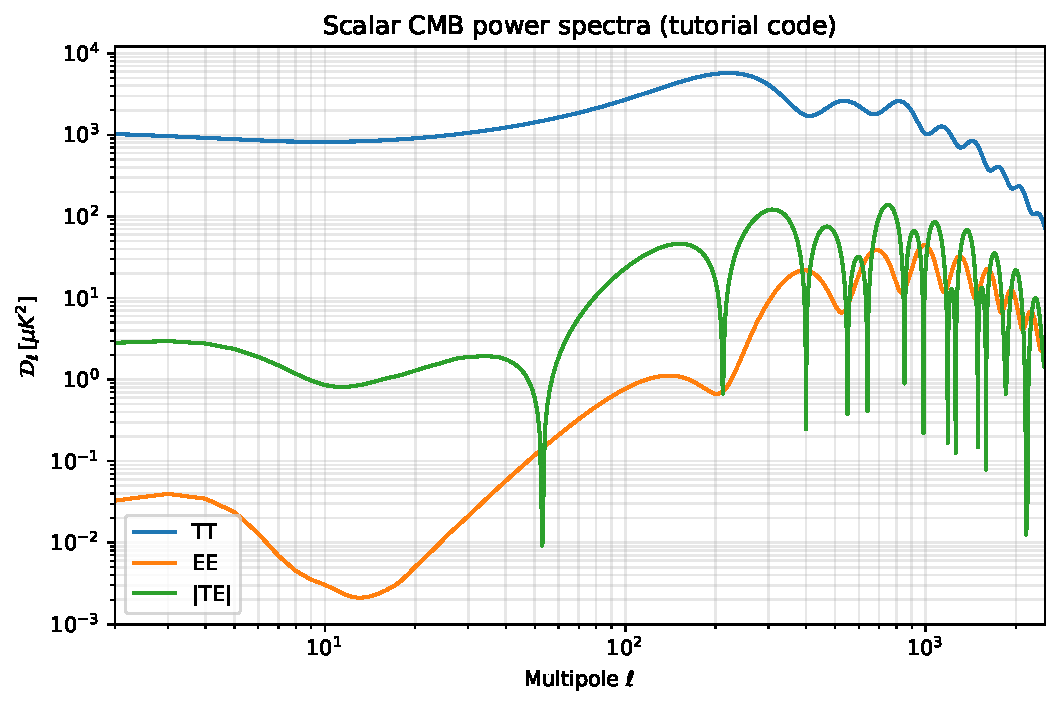
\includegraphics[width=0.85\linewidth]{figures/06_scalar_spectra.pdf}
\end{center}

\noindent Three curves: temperature TT (blue) with the Sachs-Wolfe plateau, six acoustic peaks, and the Silk damping tail; $E$-mode polarisation EE (orange) with peaks 90$^\circ$ out of phase with TT and a reionisation bump at $\ell \lesssim 10$; the temperature-polarisation cross-spectrum $|$TE$|$ (green), which oscillates between positive and negative values.

\subsection{Validation against CAMB}

We promised CAMB would only appear twice. This is the first time. Set up an equivalent CAMB run and overplot.

\begin{codebox}[Cell: compare with CAMB]
\begin{lstlisting}[style=python]
import camb
pars = camb.set_params(H0=100 * params['h'],
                       ombh2=params['omega_b_h2'],
                       omch2=params['omega_c_h2'],
                       As=params['A_s'], ns=params['n_s'],
                       tau=params['tau_reion'])
pars.set_for_lmax(params['ell_max'], lens_potential_accuracy=2)
camb_powers = camb.get_results(pars).get_cmb_power_spectra(
    pars, CMB_unit='muK', raw_cl=False)
unlensed = camb_powers['unlensed_scalar']  # shape (lmax+1, 4); cols = TT,EE,BB,TE

ells_camb = np.arange(unlensed.shape[0])
Dl_TT_camb = unlensed[:, 0]
Dl_EE_camb = unlensed[:, 1]
Dl_TE_camb = unlensed[:, 3]
\end{lstlisting}
\end{codebox}

\begin{codebox}[Cell: plot tutorial vs CAMB with residuals]
\begin{lstlisting}[style=python]
fig, axes = plt.subplots(2, 1, sharex=True, figsize=(8, 6),
                         gridspec_kw={'height_ratios': [3, 1]})

# Top: spectra
axes[0].plot(ells,      Dl_TT,                  'k-',  lw=1.4, label='tutorial')
axes[0].plot(ells_camb, Dl_TT_camb,             'C3--', lw=1.0, label='CAMB')
axes[0].plot(ells,      Dl_EE,                  'k-',  lw=1.4)
axes[0].plot(ells_camb, Dl_EE_camb,             'C3--', lw=1.0)
axes[0].set_yscale('log'); axes[0].set_xscale('log')
axes[0].set_ylabel(r'$\mathcal{D}_\ell$ [$\mu K^2$]')
axes[0].set_xlim(2, params['ell_max'])
axes[0].legend(); axes[0].grid(True, which='both', alpha=0.3)
axes[0].set_title('Validation: tutorial vs CAMB')

# Residuals
common = np.intersect1d(ells, ells_camb)
ix_t   = np.isin(ells, common)
ix_c   = np.isin(ells_camb, common)
resid_TT = 100.0 * (Dl_TT[ix_t] - Dl_TT_camb[ix_c]) / Dl_TT_camb[ix_c]
resid_EE = 100.0 * (Dl_EE[ix_t] - Dl_EE_camb[ix_c]) / Dl_EE_camb[ix_c]
axes[1].plot(common, resid_TT, 'C0-', lw=1.0, label='TT')
axes[1].plot(common, resid_EE, 'C1-', lw=1.0, label='EE')
axes[1].axhline(0, color='gray', lw=0.5)
axes[1].set_xscale('log')
axes[1].set_xlabel(r'Multipole $\ell$')
axes[1].set_ylabel('residual [%]')
axes[1].set_ylim(-5, 5)
axes[1].legend(); axes[1].grid(True, which='both', alpha=0.3)
plt.show()
\end{lstlisting}
\end{codebox}

\begin{center}
  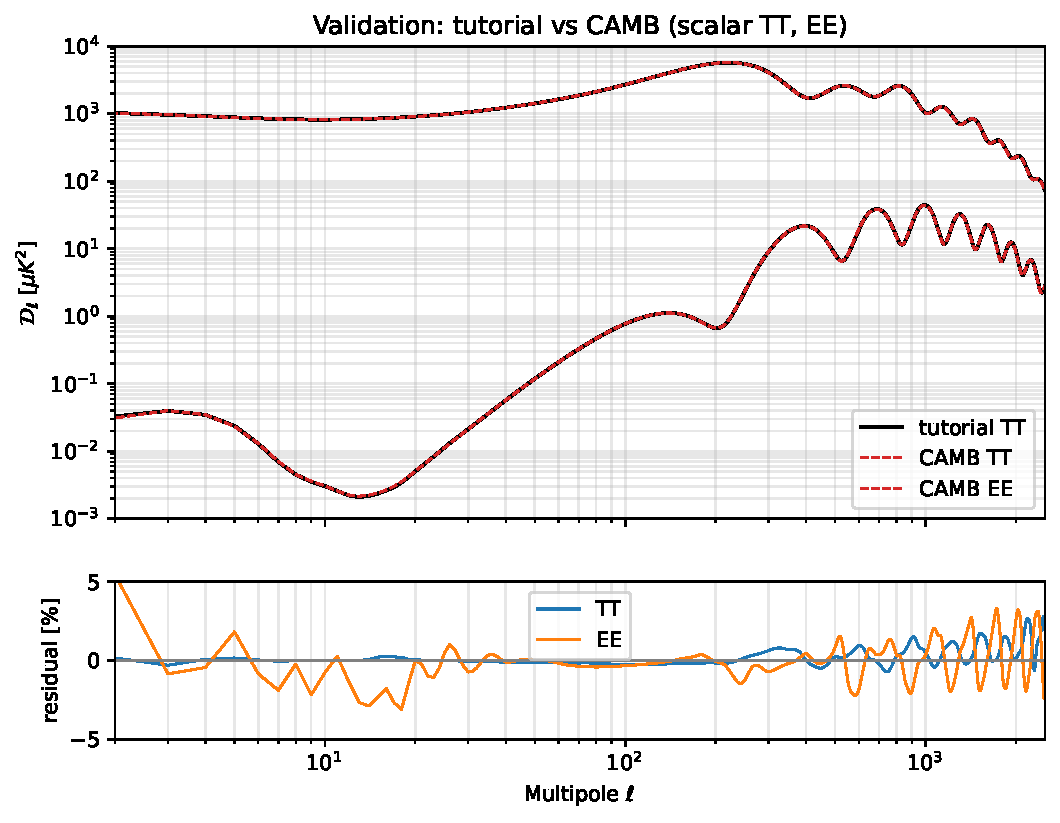
\includegraphics[width=0.85\linewidth]{figures/06b_scalar_validation.pdf}
\end{center}

\noindent Agreement at the percent level across the full $\ell$ range, with residuals localised on the acoustic peaks (mostly numerical-projection artefacts).

\subsection{Looking ahead}

These are the \emph{unlensed} scalar spectra. The real CMB has been lensed by intervening matter, which smooths the acoustic peaks and -- more importantly -- converts a fraction of the $E$-mode power into $B$-mode polarisation. That is chapter 6. After that, chapter 7 adds the contribution from primordial gravitational waves, which produce a tensor $B$-mode signal.
